\documentclass[
titlepage=firstiscover,
bibliography=totoc,
captions=tableheading,
]{scrartcl}

\usepackage[aux]{rerunfilecheck}



\usepackage{polyglossia}
\usepackage[autostyle]{csquotes}
\setmainlanguage{german}
\setotherlanguages{english, french}

\usepackage{microtype}

\usepackage{amsmath}
\usepackage{amssymb}
\usepackage{mathtools}

\usepackage{fontspec}

\usepackage[
  style=alphabetic,
]{biblatex}
\addbibresource{main.bib}

\usepackage[
math-style=ISO,
bold-style=ISO,
sans-style=italic,
nabla=upright,
partial=upright,
]{unicode-math}

\usepackage[
  locale=DE,
  separate-uncertainty=true,
  per-mode=symbol-or-fraction,
]{siunitx}

\sisetup{
locale=DE,
per-mode=symbol-or-fraction}

\usepackage[unicode]{hyperref}
\usepackage{bookmark}

\usepackage{graphicx}
\graphicspath{{build/}}

\usepackage{caption, booktabs}

\usepackage{grffile}
\usepackage{subcaption}
\usepackage{float}

\usepackage{xfrac}


\begin{document}

  \section{Aufgabe 13}
    \subsection{Aufgabe 13a}

    \begin{align*}
      E &\coloneq \frac{E}{\symup{TeV}}\\
      \phi &= \phi_0\cdot(E)^{-\gamma}\\
      \gamma' &\coloneq -\gamma\\
      \implies\,\,\, 1&=\int_1^\infty \phi_0E^{+\gamma'}\,dE=
      \left[\phi_0\frac1{\gamma'+1}E^{\gamma'+1}\right]_1^\infty=-\phi_0
      \frac1{\gamma'+1}\\
      \iff \phi_0&=-(\gamma'+1)\\
      \,\\
      F&=-(\gamma'+1)\int_1^E E^{\gamma'}\,dE \\
      &=-(\gamma'+1)\left[\frac1{\gamma'+1}E^{\gamma'+1}\right]_1^E\\
      &=-(\gamma'+1)\left[\frac1{\gamma'+1}\cdot E^{\gamma'+1}\right]_1^E\\
      &=-(\gamma'+1)\left(\frac1{\gamma'+1}\cdot E^{\gamma'+1}-\frac1{\gamma'+1}\right)\\
      &=-E^{\gamma'+1}+1\\
      &=1-E^{-1,7}=u\\
      \implies &E^{-1,7}=1-u \iff E=(1-u)^{-\frac1{1,7}}
    \end{align*}






  \section{Aufgabe 14}
    \subsection{Aufgabe 14a}
    Scatterplot für die ersten zwei Dimensionen des Datensatzes:
    \begin{figure}[H]
      \centering
      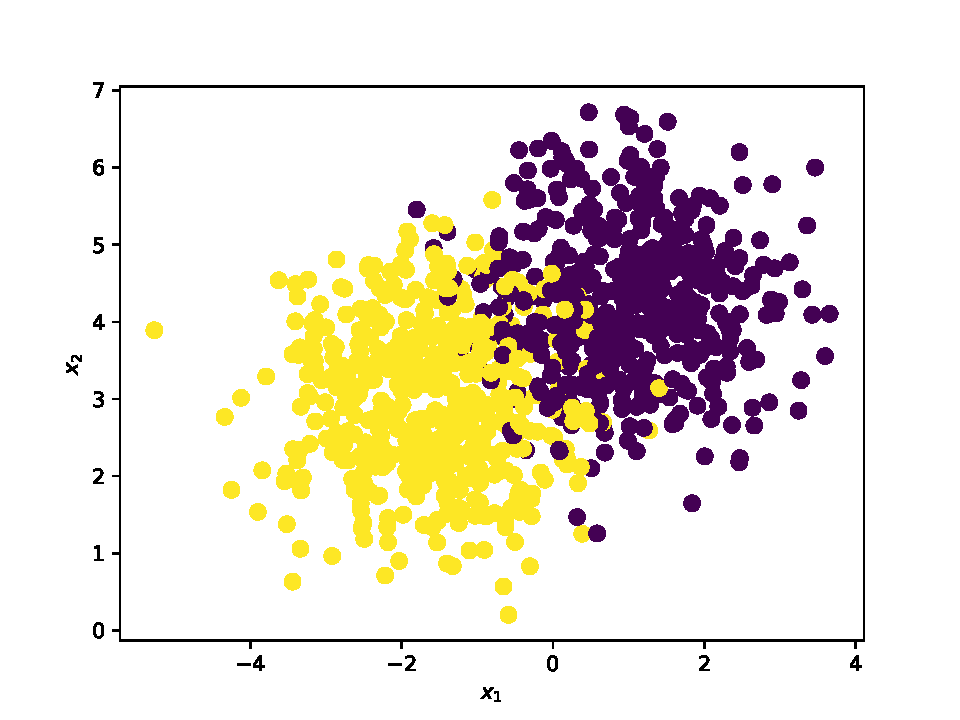
\includegraphics[height=7cm]{a_scatter.pdf}
      \caption{Scatterplot von $x_1$ und $x_2$.}
      \label{fig:ascatter}
    \end{figure}

    \subsection{Aufgabe 14b}
    Die Hauptkomponentenanalyse sucht nach einer Basis im Raum indem die Varianz entlang der Basisvektoren maximiert wird.\\
    Gegeben seien also N
    Datenpunkte mit d Dimensionen.

    \begin{enumerate}
      \item Zentrierung
        \begin{enumerate}
          \item Mittelwertvektor $\mu$ bilden.
          \begin{align*}
            \mu =
            \begin{pmatrix*}[c]
              \bar{x_1}\\
              \bar{x_2}\\
              \bar{x_3}\\
              \bar{x_4}\\
            \end{pmatrix*}
          \end{align*}
          \item $x_i\, = x_i - \mu$
        \end{enumerate}
      \item Kovarianz
        \begin{enumerate}
          \item Kovarianzmatrix Cov($\symbf{X}$) bilden
        \end{enumerate}
      \item Eigenwerte und Vektoren
        \begin{enumerate}
          \item Die 4 Eigenwerte und Eigenvektoren von Cov($X$) bestimmen, und der Größe nach sortieren.
        \end{enumerate}
      \item Transformierung
        \begin{enumerate}
        \item  Den Datensatz $\symbf{X}$ mit der Transformationsmatrix $\symbf{W}$ aus den        Eigenvektoren multiplizieren.
          \begin{align*}
            \symbf{X}\' = \symbf{X}\symbf{W}
          \end{align*}
          Es ergibt sich die transformierte Matrix $\symbf{X}\'$
        \end{enumerate}
    \end{enumerate}

    \subsection{Aufgabe 14c}
    Die Eigenwerte der Kovarianzmatrix ergeben sich zu:
    \begin{align*}
      \lambda_1 &= 17.519\\
      \lambda_2 &= 0.999\\
      \lambda_3 &= 0.988\\
      \lambda_4 &= 0.899\\
    \end{align*}
    Es ist deutlich dass der erste Eigenwert eine wesentlich höhere Korrelation als
    die anderen beschreibt.

    \subsection{Aufgabe 14d}
    \begin{figure}[H]
      \centering
      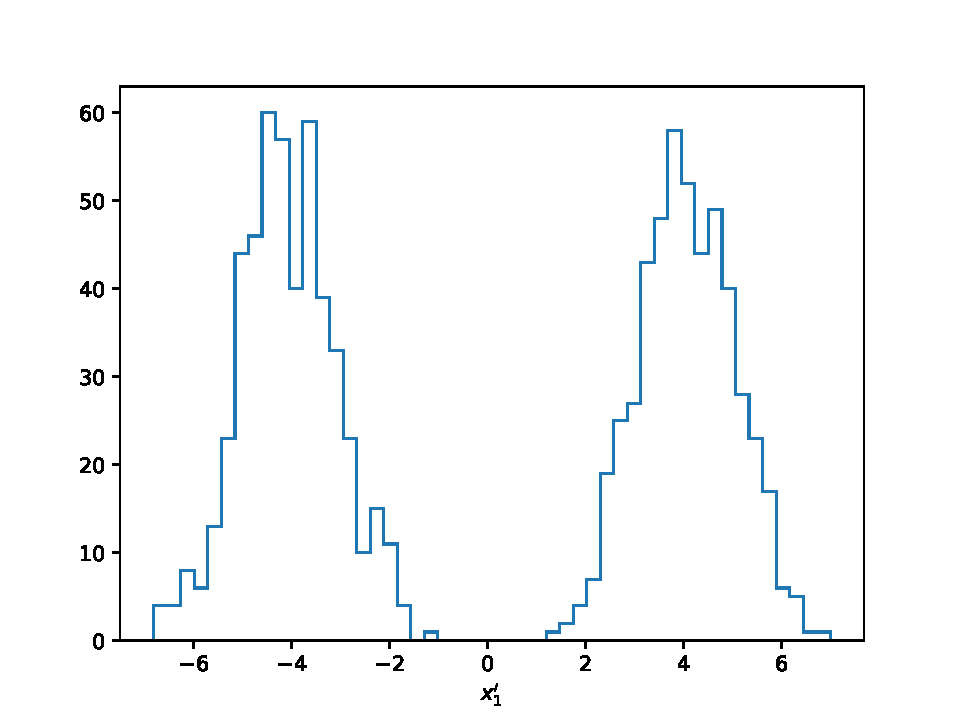
\includegraphics[height=7cm]{d_histx1.pdf}
      \caption{Histogramm von $x_1\'$.}
      \label{fig:dhistx1}
    \end{figure}
    \begin{figure}[H]
      \centering
      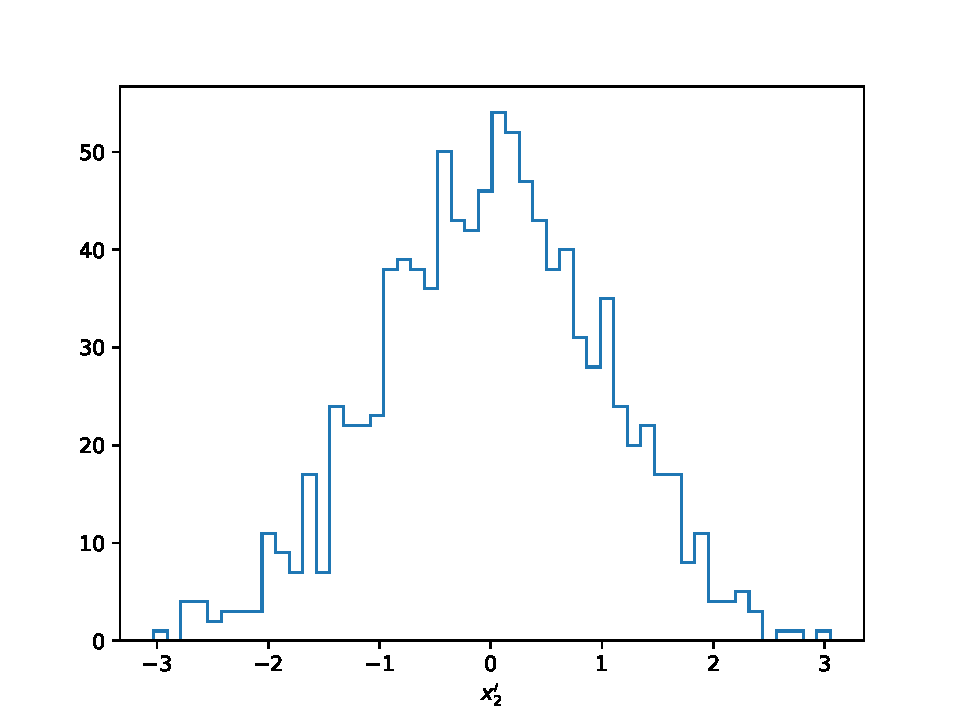
\includegraphics[height=7cm]{d_histx2.pdf}
      \caption{Histogramm von $x_2\'$.}
      \label{fig:dhistx2}
    \end{figure}
    \begin{figure}[H]
      \centering
      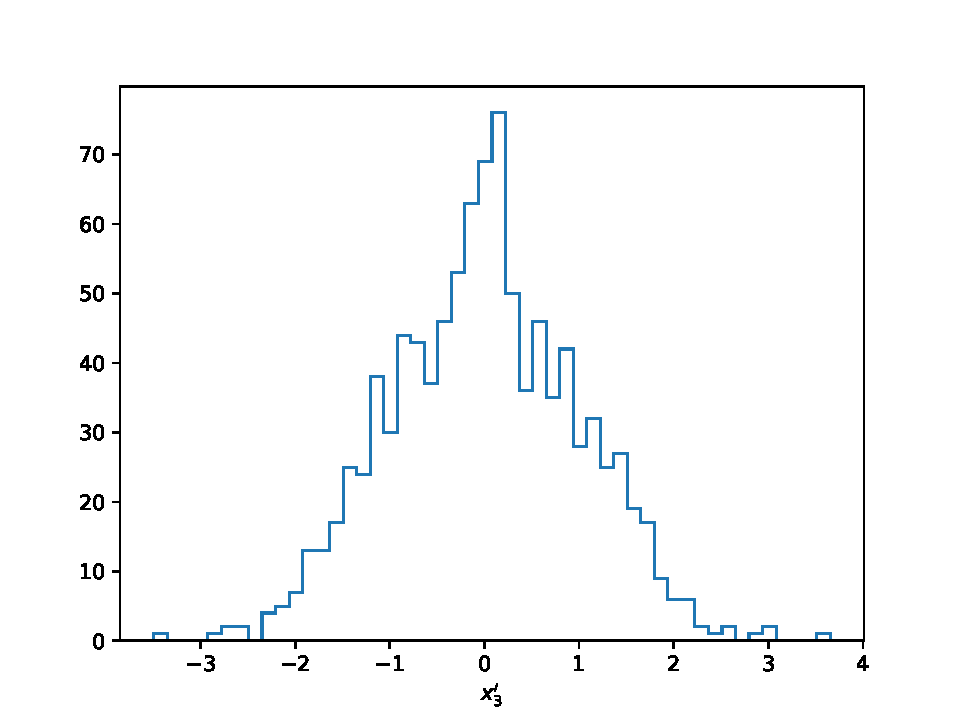
\includegraphics[height=7cm]{d_histx3.pdf}
      \caption{Histogramm von $x_3\'$.}
      \label{fig:dhistx3}
    \end{figure}
    \begin{figure}[H]
      \centering
      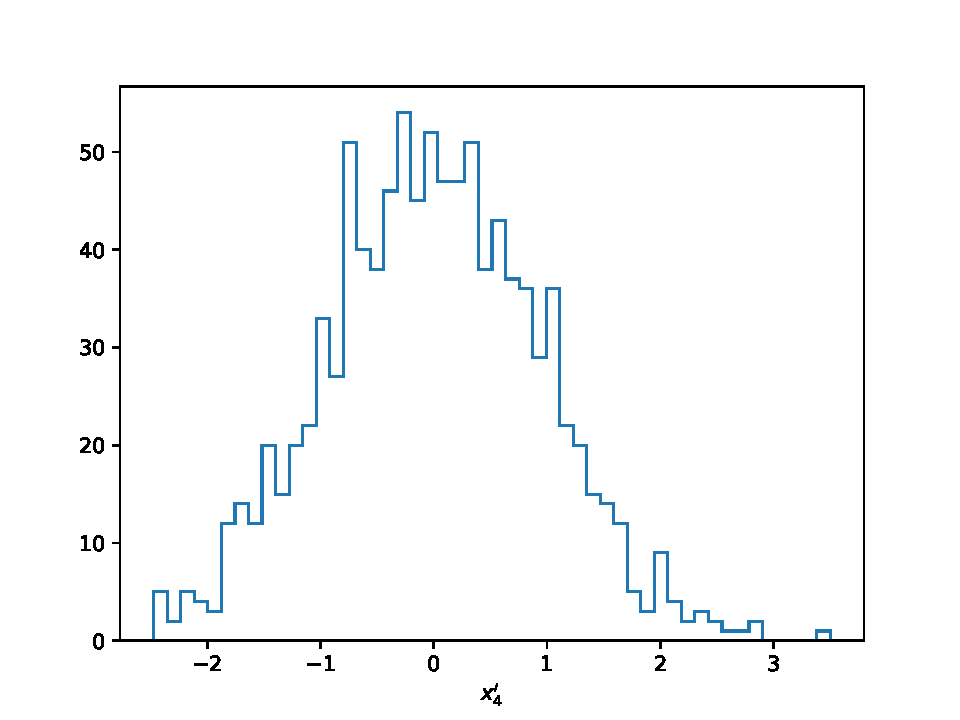
\includegraphics[height=7cm]{d_histx4.pdf}
      \caption{Histogramm von $x_4\'$.}
      \label{fig:dhistx4}
    \end{figure}
    \begin{figure}[H]
      \centering
      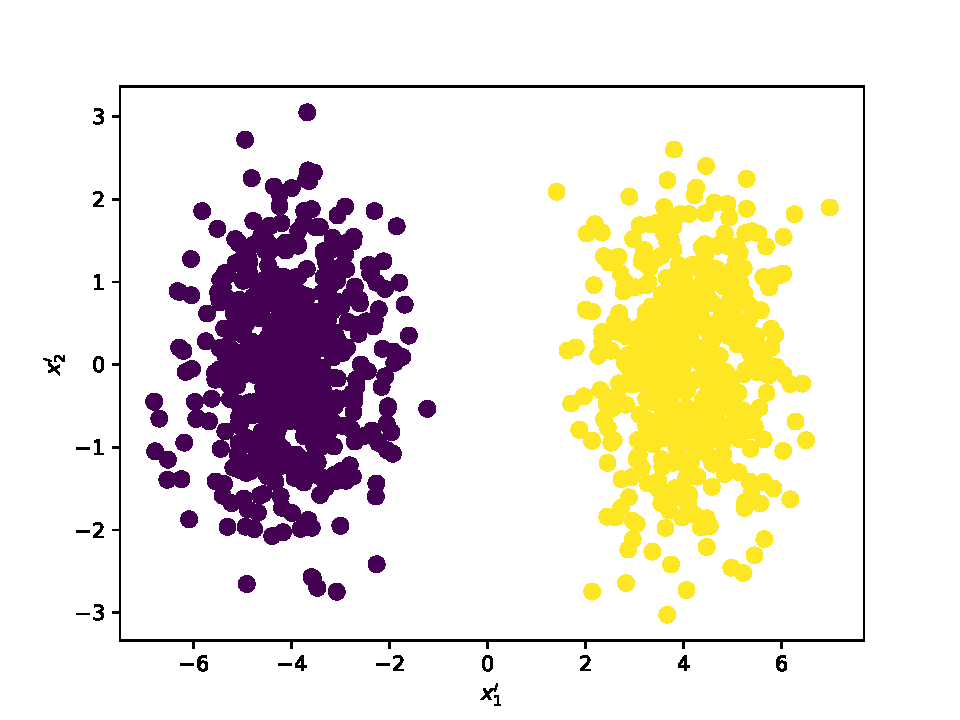
\includegraphics[height=7cm]{d_scatterx1x4.pdf}
      \caption{Scatterplot von $x_1\'$ und $x_2\'$.}
      \label{fig:dscatter}
    \end{figure}

\end{document}
